\documentclass[a4paper,12pt]{article}

\usepackage{mystyle}
\usepackage{gensymb}


\usepackage{scalerel}
\usepackage{stackengine}

\graphicspath{ {images/} }


% https://tex.stackexchange.com/questions/5461/is-it-possible-to-change-the-size-of-an-arrowhead-in-tikz-pgf
\usetikzlibrary{arrows.meta}


\DeclareMathOperator{\Image}{Im}

\definecolor{pink}{RGB}{218, 3, 174}
\definecolor{violet}{RGB}{148, 0, 211}
\definecolor{green}{RGB}{0, 153, 0}
\definecolor{orange}{RGB}{255, 153, 0}
\definecolor{blue}{RGB}{5, 73, 255}


% https://tex.stackexchange.com/a/101138/135045

\newcommand\widesim[1]{\ThisStyle{%
  \setbox0=\hbox{$\SavedStyle#1$}%
  \stackengine{-.1\LMpt}{$\SavedStyle#1$}{%
    \stretchto{\scaleto{\SavedStyle\mkern.2mu\sim}{.5150\wd0}}{.6\ht0}%
  }{O}{c}{F}{T}{S}%
}}

\newcommand{\BigMiddleThree}{\;\left|\vphantom{\begin{pmatrix} 0\\0\\0 \end{pmatrix}}\right.\;}
\newcommand{\BigMiddleFour}{\;\left|\vphantom{\begin{pmatrix} 0\\0\\0\\0 \end{pmatrix}}\right.\;}


% https://tex.stackexchange.com/questions/63531/how-to-write-quotation-marks-in-math-environment
\DeclareMathSymbol{\mlq}{\mathord}{operators}{``}
\DeclareMathSymbol{\mrq}{\mathord}{operators}{`'}


\DeclareMathOperator{\Imag}{Im}


% https://tex.stackexchange.com/questions/544453/undefined-control-sequence-after-paragraph
\renewcommand{\paragraph}[1]{\noindent\textbf{#1}\quad}


% https://tex.stackexchange.com/questions/36851/skipping-line-after-proof-in-proof-environment#comment73553_36851
\newcommand{\proofindent}{\hspace*{\fill}\par\vspace{0.5em}\noindent}



\author{Алексеев Василий}


\title{Семинар 7}
\date{24 + 28 марта 2023}


\begin{document}
  \maketitle
  
  \tableofcontents

  \thispagestyle{empty}
  
  \newpage
  
  \pagenumbering{arabic}


  \section{Diag 1. Часть 1}
  
  \subsection{Диагонализируемость отображения}
  
  Пусть есть линейное преобразование $\phi\colon X \hm\to Y$, где $X$ и $Y$ есть линейные пространства размерностей~$n$ и $m$ соответственно.
  Выберем базисы в пространствах $X$ и $Y$: $e \hm= (\bds e_1, \ldots, \bds e_n)$ в $X$ и $f \hm= (\bds f_1, \ldots, \bds f_m)$ в $Y$.
  В паре базисов $e$ и $f$ линейному преобразованию $\phi$ соответствует матрица~$A \hm\in \RR^{m\times n}$.
  Если выбрать другие базисы: $e' = (\bds e_1', \ldots, \bds e_n')$ и $f' = (\bds f_1', \ldots, \bds f_m')$~---~то матрица $A'$ \emph{того же самого} преобразования $\phi$ в этой паре базисов будет \emph{другой}.
  Можно ли выбрать базисы $e'$ и $f'$ так, чтобы матрица $A'$ оказалась ``хорошей''?
  Например, чтобы она была \emph{диагональной}?
  
  Попробуем найти такие базисы $e'$ и $f'$.
  Пусть $\bds e_1'$~---~просто какой-нибудь ненулевой вектор.
  Посмотрим на его образ $\phi(\bds e_1')$.
  Если $\phi(\bds e_1') \hm= \bds 0$, то первый столбец~$A'$ будет нулевым (это хорошо, пока матрица получается диагональной).
  Если же $\phi(\bds e_1') \hm{\not=} \bds 0$, то положим $\bds f_1' \hm\equiv \phi(\bds e_1')$.
  В таком случае первый столбец~$A'$ будет первым столбцом единичной матрицы.
  В любом случае, первый столбец~$A'$ можно сделать ``хорошим''.
  
  Далее, выберем $\bds e_2'$~---~какой-нибудь такой, чтоб система $(\bds e_1', \bds e_2')$ была линейно независимой (считаем $n \hm\geq 2$).
  И снова смотрим на образ $\phi(\bds e_2')$.
  Если $\phi(\bds e_2') \hm= \bds 0$, то опять больше ничего делать не надо: второй столбец~$A'$ нулевой.
  Если же $\phi(\bds e_2') \hm{\not=} \bds 0$, то... можно ли этот образ выбрать вторым базисным $\bds f_2'$?
  Можно, но только если $(\bds f_1', \bds f_2')$ будут линейно независимыми!
  Итого, имеем две возможности при ненулевом $\phi(\bds e_2')$: он линейно независим с выбранным ранее $\bds f_1'$ (или если на предыдущем шаге первого нового базисного в $Y$ вообще выбрано не было) или же раскладывается по нему (то есть коллинеарен).
  Если $\phi(\bds e_2')$ и $\bds f_1'$ линейно независимы, то поступаем как в прошлый раз при ненулевом $\phi(\bds e_1')$: берём $\bds f_2' \hm\equiv \phi(\bds e_2')$ и получаем второй столбец $A'$ как у единичной матрицы.
  Если $\phi(\bds e_2')$ и $\bds f_1'$ линейно зависимы, то это значит, что найдётся $\alpha \hm\in \RR$, такой что:
  \[
    \phi(\bds e_2') = \alpha \bds f_1' \leftrightarrow \phi(\bds e_2') = \alpha \phi(\bds e_1')
  \]
  ``Несложно заметить'', что можно ``поправить'' вектор $\bds e_2'$.
  Поправить так, чтобы занулить его образ:
  \[
    \bds e_2'' \equiv \bds e_2' - \alpha \bds e_1'
    \Rightarrow \phi(\bds e_2'') = \phi(\bds e_2' - \alpha \bds e_1') = \phi(\bds e_2') - \alpha \phi(\bds e_1') = \bds 0
  \]
  При этом векторы $(\bds e_1', \bds e_2'')$, очевидно, линейно независимы (так как получены невырожденной заменой из пары линейно независимых векторов $(\bds e_1', \bds e_2')$).
  А второй столбец $A'$ получается нулевым.
  (Чтобы не усложнять обозначения, далее будем называть второй вектор просто $\bds e_2'$, то есть с одним ``штрихом''~---~вне зависимости от того, пришлось ли вносить ``правку'' или нет.)
  В любом случае~---~удалось продолжить поиск базисов в $X$ и $Y$ так, чтобы матрица~$A'$ получалась диагональной (первые два столбца уже ``хорошие'').
  
  Несложно увидеть, что далее процесс поиска базисных векторов $e'$ и $f'$ продолжается точно так же, как с вектором~$\bds e_2'$~(\ref{fig:map-x-y-diag-scheme}).
  Например, далее надо бы было взять $\bds e_3'$ такой, чтоб он был линейно независим с $\bds e_1'$ и $\bds e_2'$.
  Его образ $\phi(\bds e_3')$ либо нулевой, либо ненулевой и \textbf{не} раскладывается по уже выбранным первым базисным $f'$ (в таком случае $\phi(\bds e_3')$ можно взять в качестве следующего базисного в $Y$), либо он ненулевой и раскладывается по имеющимся первым базисным $f'$ (в этом случае, пользуясь линейностью~$\phi$, можно ``поправить'' $\bds e_3'$, сделав его образ нулевым).
  
  \begin{figure}[h]
    \centering
  
    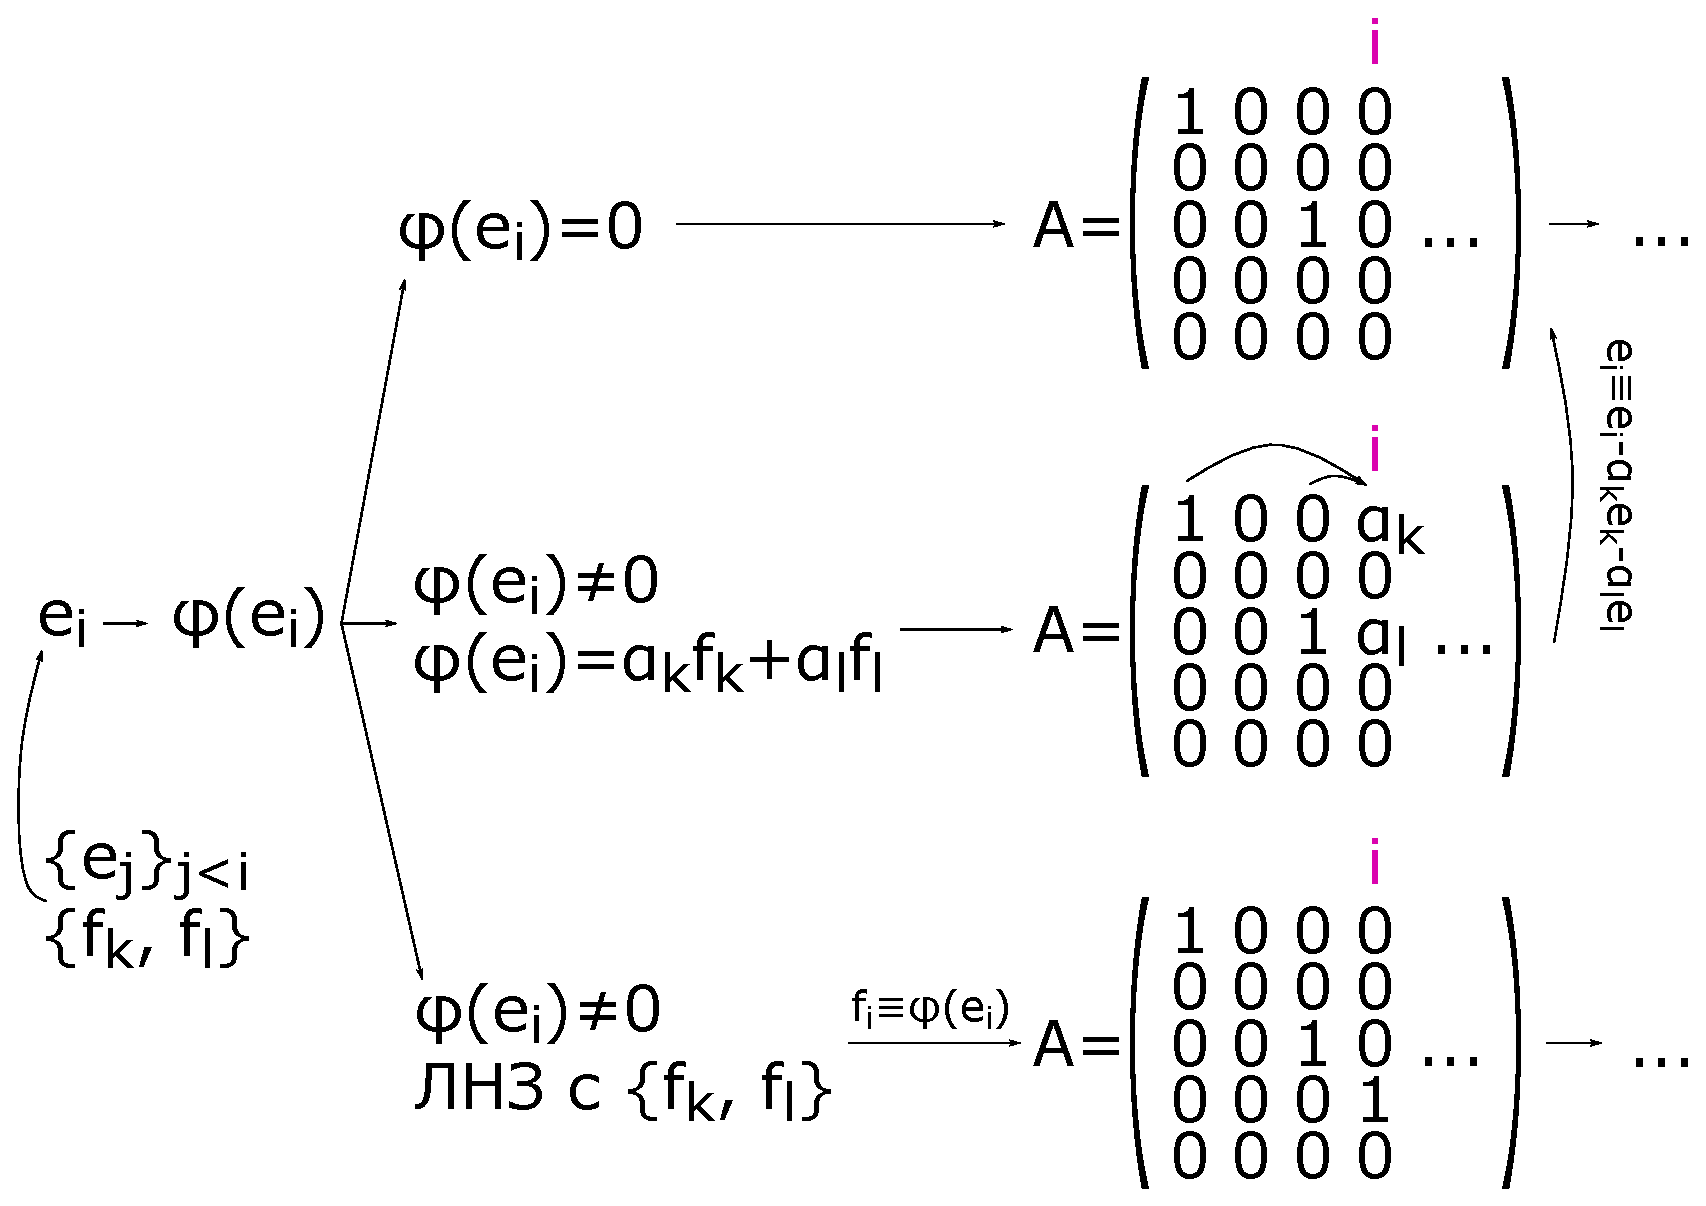
\includegraphics[width=0.9\columnwidth]{map-x-y-diag-scheme}
  
    \caption{Выбор очередного вектора $e_i$ для базиса $e$ в $X$ (и, возможно, также $f_i$ для базиса $f$ в $Y$), так чтобы матрица~$A$ отображения $\phi\colon X \hm\to Y$ была диагональной.}
    \label{fig:map-x-y-diag-scheme}
  \end{figure}
  
  В результате описанного процесса получаем базис $e' \hm= (\bds e_1', \ldots, \bds e_n')$ в $X$ и... возможно, ``недостроенный'' базис $(\bds f_1', \ldots, \bds f_r')$, $r \hm\leq m$.
  Возможно, недостроенный~---~хотя бы потому, что не при любом исходе удавалось выбрать вектор в $f'$ при выборе очередного вектора в $e'$ (могло бы в принципе получиться и так, что ни одного $f'$ вообще не было выбрано~---~если всегда оказывались нулевые столбцы в $A'$).
  Но линейно независимую систему $(\bds f_1', \ldots, \bds f_r')$, если в ней недостаточно векторов, всегда можно достроить до базиса в~$Y$, выбрав ``как-нибудь'' оставшиеся $m \hm- r$ векторов (так, чтобы система из уже $m$ векторов тоже была линейно независимой).
  
  Итого, нашли базисы $e'$ и $f'$ в $X$ и $Y$, такие что матрица~$A'$ отображения $\phi\colon X \hm\to Y$ в них имеет диагональный вид: только на её главной диагонали $\{a_{ii} \hm\mid i \hm= 1, \ldots, \min(m, n)\}$, возможно, стоят ненулевые значения (причём даже если $a_{ii} \hm{\not=} 0$, то обязательно $a_{ii} \hm= 1$).
  Сколько будет единиц на диагонали~$A'$?
  Их число определяет количество линейно независимых столбцов $A'$.
  Эти столбцы (точнее, соответствующие им векторы в $Y$) составляют базис в $\Imag \phi$.
  Таким образом, единиц на диагонали~$A'$ всего $\dim \Imag \phi$ штук.
  Далее, перенумеровкой векторов $e'$ можно добиться того, чтоб единицы на диагонали $A'$ шли подряд начиная с начала.
  В итоге $A'$ будет иметь вид:
  \begin{equation}\label{eq:matrix-diag-view}
    %A' = \diag\ (
      %\hphantom{\hspace{0.5em}}\underbrace{\hphantom{1}1, \ldots, 1\hphantom{1}}_{\dim\Imag\phi}
      %\underbrace{\hphantom{1}0, \ldots, 0\hphantom{1}}_{\dim X - \dim\Imag\phi}
    %)  % TODO: phantoms... UPD: and this is not quite "diag"...
    A' = (a'_{ij})_{\substack{1 \leq i \leq m\\ 1 \leq j \leq n}},\quad \left\{
      \begin{aligned}
        &a'_{ij} = 1,\quad 1 \leq i = j \leq \dim\Imag\phi\\
        &a'_{ij} = 0,\quad \mbox{иначе}
      \end{aligned}
    \right.
  \end{equation}
  
  Раз в $X$ и $Y$ фактически прошла замена базисов~---~от ``старых'' $e$ и $f$ к ``новым'' $e'$ и $f'$~---~то можно ввести ещё матрицы перехода $S \hm\in \RR^{n\times n}$ и $P \hm\in \RR^{m\times m}$:
  \[
    e' = e S,\quad f' = f P
  \]
  где $e'$ и $e$ это строчки, каждая из $n$ векторов пространства $X$, то есть $e, e' \hm\in X^{1\times n}$,~---~а $f$ и $f'$ это строчки $Y^{1\times m}$.
  Но тогда связь между ``старой'' и ``новой'' матрицами отображения $\phi$ есть:
  \begin{equation}\label{eq:matrix-change1}
    A' = P^{-1} A S
  \end{equation}
  
  Всё выше описанное выливается в такие два утверждения.
  
  \begin{theorem}
    Для любого линейного преобразования $\phi\colon X \hm\to Y$ найдётся пара базисов $e'$ и $f'$ в пространствах $X$ и $Y$ соответственно, такая что матрица преобразования $A'$ будет диагональной вида~(\ref{eq:matrix-diag-view}). 
  \end{theorem}
  
  \begin{theorem}
    Для любой матрицы $A \hm\in \RR^{m \times n}$ найдётся пара невырожденных квадратных матриц $S \hm\in \RR^{n\times n}$ и $P \hm\in \RR^{m\times m}$, таких что матрица $A' \hm= P^{-1} A S$ будет диагональной вида~(\ref{eq:matrix-diag-view}). 
  \end{theorem}
  
  
  \subsection{Собственные векторы и собственные значения}
  
  Пусть теперь есть \emph{преобразование} $\phi\colon X \hm\to X$.
  Если в $n$-мерном пространстве $X$ выбран базис $e$, то преобразованию будет соответствовать матрица $A \hm\in \RR^{n\times n}$.
  Можно ли выбрать базис $e'$ так, чтобы матрица преобразования в нём $A'$ была диагональной?
  Изменение матрицы преобразования при смене базиса $e' \hm= e S$ описывается формулой:
  \begin{equation}\label{eq:matrix-change2}
    A' = S^{-1} A S
  \end{equation}
  Сравнивая с формулой изменения матрицы отображения~(\ref{eq:matrix-change1}), несложно заметить, что в случае преобразования \emph{возможностей для изменения матрицы меньше}: вместо двух матриц $S$ и $P$ теперь всего одна $S$.
  Поэтому кажется, что \emph{подходящий базис $e'$ для приведения матрицы преобразования $\phi$ к диагональному виду получится найти не всегда}.
  
  Когда его можно будет найти?
  И как его найти?
  Попробуем выяснить, какими свойствами должны обладать векторы подходящего базиса.
  Пусть найден базис $e'$, в котором матрица преобразования $A'$ диагональна: $A' \hm= \diag(\lambda_1, \ldots, \lambda_n)$, $\lambda_i \hm\in \RR$ (даже не требуем только единиц на диагонали~---~просто диагональный вид).
  Но в таком случае:
  \begin{equation}\label{eq:imag-parall-orig}
    \left\{
      \begin{aligned}
        &\phi(\bds e_i') = \lambda_i \bds e_i'\\
        &i = 1, \ldots, n
      \end{aligned}
    \right.
  \end{equation}
  то есть \emph{образ $\phi(\bds e_i')$ каждого базисного вектора $\bds e_i'$ оказывается параллелен этому же $\bds e_i'$}!
  
  Можно ли вообще для преобразования $\phi$ найти векторы, обладающие свойством~(\ref{eq:imag-parall-orig})?
  То есть найдутся ли число $\lambda \in \RR$, вектор $\bds x \in X$, такие что
  \begin{equation}\label{eq:eigenvector}
    \phi(\bds x) = \lambda \bds x
  \end{equation}
  
  \begin{definition}
    Вектор $\bds x \hm\in X$ называется \emph{собственным вектором} преобразования $\phi\colon X \hm\to X$, соответствующим \emph{собственному значению} $\lambda \hm\in \RR$, если 1) вектор $\bds x$ ненулевой и 2) $\phi(\bds x) \hm= \lambda \bds x$.
  \end{definition}
  
  Перепишем выражение~(\ref{eq:eigenvector}) в терминах матриц и вектор-столбцов (матрица $A$ есть матрица преобразования $\phi$ в ``старом'' базисе $e$, а $x \hm\in \RR^n$ есть координатный столбец вектора $\bds x \hm\in X$):
  \begin{equation}\label{eq:imag-parall-orig-in-matrix-form}
    Ax = \lambda x \leftrightarrow \boxed{(A - \lambda E) x = 0}
  \end{equation}
  
  Когда будет иметь \textbf{нетривиальное} решение уравнение~(\ref{eq:imag-parall-orig-in-matrix-form})?
  В том случае, если определитель системы отличен от нуля:
  \begin{equation}\label{eq:characteristic-equation}
    \boxed{
      \det(A - \lambda E) = 0
    }
  \end{equation}
  
  Уравнение~(\ref{eq:characteristic-equation}) называется \emph{характеристическим уравнением} матрицы $A$.
  Из него можно найти собственные значения, а далее из системы~(\ref{eq:imag-parall-orig-in-matrix-form}) найти собственные вектора.
  
  Заметим ``что-нибудь интересное'' в уравнении~(\ref{eq:characteristic-equation}).
  Начнём по-честному его расписывать.
  И воспользуемся для этого формулой полного разложения определителя.
  Итак, пусть $A \hm= \left(\begin{smallmatrix} a_{11} & \ldots & a_{1n} \\ \vdots & \ddots & \vdots \\ a_{n1} & \ldots & a_{nn}\end{smallmatrix}\right)$.
  Тогда уравнение~(\ref{eq:characteristic-equation}) можно расписать так:
  \begin{equation}
  \begin{split}
    \det(A - \lambda E) &= \begin{vmatrix}
      a_{11} - \lambda & \ldots & a_{1n}\\
      \vdots           & \ddots & \vdots\\
      a_{n1}           & \ldots & a_{nn} - \lambda
    \end{vmatrix}
    = \sum_{(j_1, \ldots, j_n)} (-1)^{N(j_1, \ldots, j_n)} a_{1j_1} \cdot \ldots \cdot a_{nj_n}\\
    &= (a_{11} - \lambda) \cdot \ldots \cdot (a_{nn} - \lambda) + \ldots
    = (-1)^n \lambda^n + (-1)^{n-1} \lambda^{n-1} \Sp A + \ldots + \det A
  \end{split}
  \end{equation}
  то есть это уравнение степени $n$ относительно $\lambda$ (а потому у него не более $n$ вещественных корней), причём в коэффициенте при $\lambda^{n-1}$ есть \emph{след матрицы $\Sp A$}, а свободный член равeн просто $\det A$ (то, что получается из~(\ref{eq:characteristic-equation}) в случае, если $\lambda$ ``нет'').
  
  Вернёмся к задаче, чего вообще хотим найти: линейно независимую систему из $n$ векторов, обладающих свойством~(\ref{eq:imag-parall-orig}).
  Заметим следующее:
  
  \begin{proposition}\label{theo:eigenvectors-independent}
    Собственные векторы $\bds x_1, \ldots, \bds x_k$, соответствующие \emph{различным} собственным значениям $\lambda_1, \ldots, \lambda_k$, \emph{линейно независимы}.
  \end{proposition}
  
  \begin{proof}
    Допустим противное: что векторы на самом деле линейно зависимы:
    \[
      \left\{
        \begin{aligned}
          &\alpha_1 \bds x_1 + \ldots + \alpha_k \bds x_k = \bds 0\\
          &\alpha_1^2 + \ldots + \alpha_k^2 > 0
        \end{aligned}
      \right.
    \]
    
    Заметим, что если вектор $x$ собственный, соответствующий собственному значению~$\lambda$, то и вектор $\alpha \bds x$ собственный ($\alpha \hm{\not=} 0$), соответствующий тому же собственному значению~$\lambda$:
    \[
      Ax = \lambda x \Rightarrow A (\alpha x) = \lambda (\alpha x)
    \]
    
    Поэтому можно считать, что ``от противного'' означает просто следующее:
    \[
      \bds x_1 + \ldots + \bds x_k = \bds 0
    \]
    
    Разберём доказательство на примере $k \hm= 3$.
    (Для произвольного $k$ всё будет аналогично, но, возможно, ещё менее наглядно.)
    \[
      \bds x_1 + \bds x_2 + \bds x_3 = \bds 0
    \]
    
    Иначе это можно переписать, выразив, например, $\bds x_3$ через $\bds x_1$ и $\bds x_2$:
    \begin{equation}\label{eq:x3-eq-x1-add-x2}
      \bds x_3 = \bds x_1 + \bds x_2
    \end{equation}
    (справа нет ``минусов'', потому что если $\bds x_1$ собственный, то $-{\bds x_1}$ тоже собственный с тем же $\lambda$~---~а для сути доказываемого не важно, собственный вектор с минусом или с плюсом).
    Подействуем преобразованием $\phi$ на обе части представленного выше соотношения~(\ref{eq:x3-eq-x1-add-x2}):
    \[
      \phi(\bds x_3) = \phi(\bds x_1 + \bds x_2) \leftrightarrow \lambda_3 \bds x_3 = \lambda_1 \bds x_1 + \lambda_2 \bds x_2
    \]
    
    Теперь подставим $\bds x_3$ из соотношения~(\ref{eq:x3-eq-x1-add-x2}):
    \[
      \lambda_3 (\bds x_1 + \bds x_2) = \lambda_1 \bds x_1 + \lambda_2 \bds x_2
      \leftrightarrow (\lambda_1 - \lambda_3) \bds x_1 + (\lambda_2 - \lambda_3) \bds x_2 = \bds 0
    \]
    
    Коэффициенты $\lambda_1 \hm- \lambda_3$ и $\lambda_2 \hm- \lambda_3$ отличны от нуля, поэтому новое соотношение ``по сути'' получается таким:
    \[
      \bds x_1 + \bds x_2 = \bds 0 \leftrightarrow \bds x_2 = -{\bds x_1}
    \]
    (``убрали'' коэффициенты, потому что если, например, $\bds x_1$ собственный, то и  $k \bds x$ при $k \hm{\not=} 0$ тоже собственный~---~а для доказываемого важно лишь, что вектор собственный).
    Но тогда вектор $-{\bds x_1}$ должен быть собственным, соответствующим тому же собственному значению, как у $\bds x_2$, то есть $\lambda_2$, хотя в то же время $-{\bds x_1}$ собственный, соответствующий $\lambda_3$.
    Так как все собственные значения по условию были различными, получаем противоречие.
    
    Рассмотрен случай трёх собственных векторов.
    Если же их больше трёх, то придётся просто несколько раз применять преобразование, постепенно уменьшая число участвуемых собственных векторов до двух.
  \end{proof}
  
  Если есть собственное значение $\lambda$, то для него найдётся хотя бы один собственный вектор (как нетривиальное решение системы~(\ref{eq:imag-parall-orig-in-matrix-form})).
  
  Приходим к следующему положению.
  
  \begin{theorem}[Достаточное условие диагонализуемости преобразования]
    \proofindent
    Если у линейного преобразования $\phi$ $n$-мерного пространства $X$ есть $n$ различных собственных значений, то найдётся базис из собственных векторов преобразования $\phi$.
    (В котором матрица преобразования будет иметь диагональный вид.)
  \end{theorem}
  
  \begin{proof}
    Можно будет найти $n$ собственных векторов, относящихся к различным собственным значениям.
    И по предложению~(\ref{theo:eigenvectors-independent}) они будут линейно независимы.
  \end{proof}
  
  
  \section{Задачи}
  
  \subsection{\# 24.20(2)}
  
  Найти собственные значения, привести к диагональному виду матрицу преобразования $\phi$, если $\phi$ есть ортогональное проектирование трёхмерного геометрического пространства векторов $\mathcal L$ на прямую $\mathcal L_1$, заданную в некотором ортонормированном базисе $e$ уравнением $\mathcal L_1\colon x\hm= y \hm= z$.
  
  \begin{solution}
    Формула преобразования $\phi$, полученная в номере 23.8(2):
    \[
      \phi(\bds x) = \frac{(\bds x, \bds a)}{|\bds a|^2} \bds a
    \]
    
    Матрица преобразования $\phi$, полученная в номере 23.9(2) (в том же базисе $e$) с помощью формулы, полученной в номере 23.8(2):
    \[
      A = \frac{1}{3} \begin{pmatrix}
        1 & 1 & 1\\
        1 & 1 & 1\\
        1 & 1 & 1
      \end{pmatrix}
    \]
    
    Теперь найдём собственные значения этой матрицы~$A$, полученной в номере 23.9(2) с помощью формулы, полученной в номере 23.8(2).
    Её характеристическое уравнение~(\ref{eq:characteristic-equation}):
    \begin{equation}
    \begin{split}
      \det(A - \lambda E) = 0
      &\leftrightarrow \left(\frac{1}{3}\right)^3 \begin{vmatrix}
        1 - 3\lambda & 1 & 1\\
        1 & 1 - 3\lambda & 1\\
        1 & 1 & 1 - 3\lambda
      \end{vmatrix} = 0\\
      &\leftrightarrow \lambda^2 (1 - \lambda) = 0
      \leftrightarrow \left\{
        \begin{aligned}
          &\lambda_1 = 0,\quad \mbox{(кратность $2$)}\\
          &\lambda_2 = 1
        \end{aligned}
      \right.
    \end{split}
    \end{equation}
    
    Теперь можно искать собственные векторы, соответствующие полученным собственным значениям $\lambda_1$\footnote{То, что ноль должен быть собственным значением, можно было заметить сразу: $\det (A \hm- \lambda E)|_{\lambda = 0} \hm= 0 \hm\leftrightarrow \det A = 0$~---~то есть наличие нулевого собственного значения равносильно тому, что матрица~$A$ вырожденная. Что и было видно.} и $\lambda_2$.
    \[
      (A - \lambda_1 E) \bds x = 0
      \leftrightarrow \begin{pmatrix}
        1 & 1 & 1\\
        1 & 1 & 1\\
        1 & 1 & 1
      \end{pmatrix} \begin{pmatrix}
        x_1 \\ x_2 \\ x_3
      \end{pmatrix} = 0
    \]
    
    Несложно сразу выписать решение системы $(A \hm- \lambda_1 E) x \hm= 0$\footnote{Видно, что в системе по сути всего одна строчка. Переменных три. Таким образом, одна переменная базисная и две свободных. То есть пространство решений системы двумерное. Поэтому достаточно хоть как-нибудь найти (хотя бы подобрать) два линейно независимых частных решения, чтобы выписать решение в общем виде.}:
    \[
      \bds x = \begin{pmatrix}
        0 \\ 1 \\ -1
      \end{pmatrix} t_1 + \begin{pmatrix}
        1 \\ -1 \\ 0
      \end{pmatrix} t_2,\quad t_1, t_2 \in \RR
    \]
    
    Видно, что собственные векторы, соответствующие $\lambda_1 \hm= 0$, образуют плоскость.
    Поэтому для $\lambda_1 \hm= 0$ можно выбрать два линейно независимых собственных вектора.
    Например:
    \[
      \bds x_1 = \begin{pmatrix}
        0 \\ 1 \\ -1
      \end{pmatrix},
      \quad \bds x_2 = \begin{pmatrix}
        1 \\ -1 \\ 0
      \end{pmatrix}
    \]
    
    Перейдём к $\lambda_2 \hm= 1$:
    \[
      (A - \lambda_2 E) \bds x = 0
      \leftrightarrow \begin{pmatrix}
        -2 & 1 & 1\\
        1 & -2 & 1\\
        1 & 1 & -2
      \end{pmatrix} \begin{pmatrix}
        x_1 \\ x_2 \\ x_3
      \end{pmatrix} = 0
    \]
    
    Сумма строчек матрицы $A \hm- \lambda_2 E$ даёт нулевую.
    А две строчки из трёх очевидно линейно независимы.
    Поэтому для того, чтобы выписать общее решение системы $(A \hm- \lambda_2 E) x \hm= 0$, достаточно подобрать всего одно нетривиальное решение.
    То есть максимальная по количеству линейно независимая совокупность собственных векторов, соответствующих $\lambda_2$, состоит из одного вектора.
    Например:
    \[
      \bds x_3 = \begin{pmatrix}
        1 \\ 1 \\ 1
      \end{pmatrix}
    \]
    
    Можно проверить, можно вспомнить~(\ref{theo:eigenvectors-independent}), но получается, что три вектора $(\textcolor{blue}{\bds x_1}, \textcolor{blue}{\bds x_2}, \textcolor{pink}{\bds x_3})$ образуют линейно независимую систему~---~нашли базис $e'$ из собственных векторов.
    В этом базисе матрица преобразования~$\phi$ примет вид:
    \[
      A' = \begin{pmatrix}
        \textcolor{blue}{\bds 0} & 0                        & 0\\
        0                        & \textcolor{blue}{\bds 0} & 0\\
        0                        & 0                        & \textcolor{pink}{\bds 1}
      \end{pmatrix}
    \]
    Именно такой~---~потому, что, например:
    \[
      \phi(\textcolor{pink}{\bds x_3}) \hm= 1 \hm\cdot \bds x_3 \hm= 0 \hm\cdot \bds x_1 \hm+ 0 \hm\cdot \bds x_2 \hm+ 1 \hm\cdot \bds x_3 \hm= (\bds x_1, \bds x_2, \bds x_3) \hm\cdot \begin{pmatrix}0 \\ 0 \\ \textcolor{pink}{\bds 1}\end{pmatrix}
    \]
    то есть в столбцы матрицы~$A'$ преобразования~$\phi$ в базисе $e' \hm= (\bds x_1, \bds x_2, \bds x_3)$ записаны координаты образов $(\phi(\bds x_1), \phi(\bds x_2), \phi(\bds x_3))$ векторов базиса $e'$ в том же базисе $e'$.
    А так как базис $e'$ состоит из собственных векторов, то матрица~$A'$ диагональная с соответствующими собственными значениями на диагонали.
    
    Можно и ``по-честному'' пересчитать матрицу преобразования в новом базисе:
    \[
      e' = (\bds x_1, \bds x_2, \bds x_3) = (\bds e_1, \bds e_2, \bds e_3) \begin{pmatrix}
        0  & 1  & 1\\
        1  & -1 & 1\\
        -1 & 0  & 1
      \end{pmatrix} = e S
    \]
    \[
      A' = S^{-1} A S = \frac{1}{3} \begin{pmatrix}
        1 & 1 & -2\\
        2 & -1 & -1\\
        1 & 1 & 1
      \end{pmatrix} \cdot \frac{1}{3} \begin{pmatrix}
        1 & 1 & 1\\
        1 & 1 & 1\\
        1 & 1 & 1
      \end{pmatrix} \cdot \begin{pmatrix}
        0  & 1  & 1\\
        1  & -1 & 1\\
        -1 & 0  & 1
      \end{pmatrix} = \begin{pmatrix}
        0 & 0 & 0\\
        0 & 0 & 0\\
        0 & 0 & 1
      \end{pmatrix}
    \]
  \end{solution}
  
  
  % \subsection{\# 24.42(1)}
  
\end{document}
